%!TEX TS-program = xelatex
%!TEX encoding = UTF-8 Unicode
\documentclass[a4paper]{report}
%\usepackage[date=short,backend=biber]{apa}
\usepackage[hidelinks]{hyperref}
\usepackage{apacite}
\usepackage[dutch]{babel}
\usepackage[a4paper, left=1in, right=1in, top=1in, bottom=.8in]{geometry}
\usepackage[utf8]{inputenc}
\usepackage{fancyhdr}
\usepackage{nameref}
\usepackage{helvet}
\usepackage{titlesec}
\usepackage{geometry}
\usepackage{ragged2e}
\usepackage{graphicx}
\usepackage{etoolbox}
\usepackage{listings}
\usepackage{xspace}
\usepackage[table]{xcolor}
\usepackage{nameref}
\usepackage{tcolorbox}
\usepackage{textcomp}
\usepackage{colortbl}
\usepackage{tabularx}
\usepackage{float}
\usepackage[printonlyused,withpage]{acronym}
%%% Je mag zelf PWM implemetneren bij bijv peltierelement of het verwarming relais.

% Styling
\renewcommand{\rmdefault}{\sfdefault}
\pagestyle{fancy}
\patchcmd{\chapter}{\thispagestyle{plain}}{\thispagestyle{fancy}}{}{}

\fancyhf{}
\fancyhead[L]{ \turtleguard }
\fancyhead[R]{ Projectplan }
\fancyfoot[R]{\thepage}

\titleformat{\chapter}[hang]
{\normalfont\huge\bfseries}{\thechapter.}{10pt}{\huge}
\titlespacing{\chapter}{0pt}{-30pt}{20pt}

\setlength{\parindent}{0.2em}

\textwidth=400pt
\geometry{
    left=25mm
}

\renewcommand{\contentsname}{Inhoudsopgave}
%\RaggedRight % Don't 'block-justify' text

\definecolor{codegreen}{rgb}{0,0.6,0}
\definecolor{codegray}{rgb}{0.5,0.5,0.5}
\definecolor{codepurple}{rgb}{0.58,0,0.82}
\definecolor{backcolour}{rgb}{0.95,0.95,0.92}

\lstdefinestyle{mystyle}{
    backgroundcolor=\color{backcolour},   
    commentstyle=\color{codegreen},
    keywordstyle=\color{magenta},
    numberstyle=\tiny\color{codegray},
    stringstyle=\color{codepurple},
    basicstyle=\ttfamily\footnotesize,
    breakatwhitespace=false,         
    breaklines=true,                 
    captionpos=b,                    
    keepspaces=true,                 
    numbers=left,                    
    numbersep=5pt,                  
    showspaces=false,                
    showstringspaces=false,
    showtabs=false,                  
    tabsize=2
}

\lstset{style=mystyle}



% Commands
\newcommand{\teambox}{
  \begin{tcolorbox}[hbox, colback=blue!5!white,colframe=blue!75!black,
    left=.1mm, right=.1mm, top=.1mm, bottom=.1mm, fontupper=\scriptsize\sffamily]
    Team Keuze
  \end{tcolorbox}
}

\newcommand{\personalbox}{
  \begin{tcolorbox}[hbox, colback=green!5!white,colframe=green!75!black,
    left=.1mm, right=.1mm, top=.1mm, bottom=.1mm, fontupper=\scriptsize\sffamily]
    Persoonlijke Keuze
  \end{tcolorbox}
}
\newcommand{\teamchoice}[1]{
  \section[ #1 ]{#1~\mbox{\teambox}}
}

\newcommand{\personalchoice}[1]{
  \section[ #1 ]{#1~\mbox{\personalbox}}
}
\newcommand{\turtleguard}{\mbox{TurtleGuard\texttrademark}\xspace}

% Document
\begin{document}


% Title Page
\begin{titlepage}
    \begin{center}
        \vspace*{.9cm}
        \Huge
        \textbf{ Projectplan \turtleguard }\\
        \vspace{0.2cm}
        \small\textit{"Hét ultieme schild-bad voor jouw schildpad"}

        \normalsize


        
        
\includegraphics[width=0.7\textwidth]{Images/turtleguard.png}
        \vspace{1cm}
        \Large\\
        \textbf{Mede mogelijk gemaakt door} \\
        
\includegraphics[width=0.2\textwidth]{Images/logouni.png}


        \vfill
      \end{center}
        \textbf{Student:} Vincent van Setten - 1734729 \\
        \textbf{Opdrachtgever:} HU University of Applied Sciences\\
        \textbf{Datum:} \today \\
        \vspace{2cm}
\end{titlepage}


% ToC
\tableofcontents

\chapter*{Versiebeheer}
\thispagestyle{empty}  % Removes header and footer from this specific page
\begin{table}[h]
    \centering
    \begin{tabular}{|c|c|c|p{5cm}|}
        \hline
        Versie & Datum      & Changes Made  \\
        \hline
        1.1    & 2023-09-19 & Tweede Versie \\
        \hline
        1.0    & 2023-09-10 & Eerste Versie \\
        \hline
    \end{tabular}
    \caption{Versiebeheer}
\end{table}
\clearpage  % End of the page

\chapter{Het Project}
\section{Introductie}
Dit document dient als project- en testplan voor het \turtleguard systeem. Het \turtleguard systeem wordt verder in detail besproken in hoofdstuk \ref{section-product}.
Verdere hoofdstukken beschrijven de architectuur van het product, de eisen aan het product en de tests die uitgevoerd zullen worden.
Het uiteindelijke doel van dit document is het beschrijven van een regelsysteem, in dit geval \turtleguard, welke ten minste twee sensoren en actuatoren bevat. 

\section{Productomschrijving}
\label{section-product}
Huisdieren, we zijn er (bijna) allemaal gek op. Vanzelfsprekend is het dus dat we het onze vertrouwde gezelschap zo comfortabel mogelijk willen maken.
Bij de meeste huisdieren is het relatief simpel, \mbox{zoals} bij een kat of hond. Zorg voor eten, drinken en aandacht en dan zijn ze vaak wel tevreden.
\par \smallskip
Echter is het niet zo eenvoudig bij alle huisdieren. Zo ook bijvoorbeeld de muskus schildpad.
Onder de (semi-)aquatische schildpadden is dit dier nog wel vrij eenvoudig, maar toch stelt het vrij strenge eisen om comfortabel en gezond te kunnen leven.
In het drukke alledaags leven is het dan ook niet altijd een makkelijk om dit allemaal in de gaten te houden.
Het laatste wat we dan ook willen is thuis komen na een warme zomerdag naar een schildpadden soep.
\par \smallskip 
Maak daarom kennis met \turtleguard. Dit simpele, maar nuttige, product houdt de leefomgeving van uw schildpad in de gaten en zorgt er voor dat deze gezond en blij blijft.
Het systeem houdt met verschillende sensoren de kwaliteit en temperatuur van het water in de gaten. 
Zo wordt u gesignaleerd als het waterkwaliteit verslechterd en wordt de temperatuur nauw in de gaten gehouden en gereguleerd.
\par \smallskip 
Met \turtleguard hoeft u zich nooit meer druk te maken of uw schildpad zich wel comfortabel voelt in zijn schild. 

\chapter{Systeem Architectuur}
\section{Hardware}
Het systeem zal draaien op de Arduino Due. Deze microcontroller heeft genoeg pinnen om alles aan te sturen, heeft gemakkelijke interfaces voor UART en I2C. Ook heb ik ervaring met het gebruik van deze microcontroller.
De verschillende sensoren en actuatoren zullen verbonden worden met de Arduino Due. 

\subsection{Sensoren}
Ik ga gebruik maken van drie verschillende sensoren. Mijn keuzes en het gebruik van deze sensoren licht ik hieronder toe.
Dit zijn de sensoren die ik ga gebruiken.
\begin{itemize}
  \item EZO\texttrademark \space pH Circuit (pH meter)
  \item DS18B20 (Water Thermometer)
  \item Adafruit MCP9808 (Lucht Thermometer)
\end{itemize}

\subsubsection{pH meter}
Een pH meter wordt gebruikt om de zuurgraad van het water te meten. 
Voor mijn schildpad is een pH van ongeveer 6.5 tot 7.5 nodig. 

Om de pH digitaal te kunnen meten, heb ik gekozen voor de  EZO\texttrademark \space pH Circuit. 
Deze sensor is goed beschikbaar en kan gebruikt worden op 3.3v en 5v. De sensor zelf is verbonden met een breakout board, welke weer verbonden kan worden met een enkele data pin, wat het uitlezen erg eenvoudig maakt.

% \subsubsection{TDS Sensor}
% Een manier om kwaliteit van het water te testen, is het meten van deeltjes die in water oplosbaar zijn.
% Dit heet \ac{TDS}. Als de TDS waarde te hoog is, moet het water vervangen worden. 
% TDS wordt aangegeven door \ac{ppm}. Dit beschrijft hoeveel deeltjes die oplosbaar zijn in water per miljoen water deeltjes zitten. De ideale TDS ligt tussen de 125ppm en 300ppm. 

\subsubsection{Water Thermometer}
De thermometer houdt de temperatuur van het water bij. Als het water te koud is, wordt het verwarmt. Als het water te warm is, wordt het verkoeld.
De ideale temperatuur voor de muskus schildpad is ongeveer 25 \textdegree c. Het water mag zo'n 3 \textdegree c warmer of kouder zijn.

\subsubsection{Omgeving Thermometer}
Ook is er een thermometer voor de temperatuur van de omgeving. Deze wordt gebruikt om te controleren hoe warm of koud het is in de omgeving. Hiermee kunnen we kijken of we verwachten dat het water warmer of kouder gaat worden.
Als het bijvoorbeeld 35 \textdegree c is, zal het waarschijnlijk niet nodig zijn om het water te verwarmen. Als het daarentegen 15 \textdegree c is, zal het verkoelen van het water weer onnodig zijn.

Deze zal worden gebruikt in combinatie met de water temperatuur. Als bijvoorbeeld de omgevingstemperatuur 30 \textdegree c is en het water is 29 \textdegree c, zal het verwarmingselement uit moeten blijven totdat de omgevingstemperatuur weer onder de 25 \textdegree c zakt. Tot die tijd zal verkoeling nodig zijn tot het water temperatuur rond de 25 \textdegree c is.


\subsection{Actuatoren}
Binnen het project ga ik gebruik maken van een aantal actuatoren, welke worden aangestuurd door de boven genoemde sensoren.
De actuatoren zal ik hieronder verder toelichten. Ik ga de volgende actuatoren gebruiken voor mijn systeem.
\begin{itemize}
  \item Verkoelingselement, geschakeld met een relais (Hobby Aqua Cooler V2).
  \item Verwarmingselement, geschakeld met een relais (Exo Terra Turtle Heater(50w)).
  \item pH Dosering pomp, geschakeld met een relais (Adafruit Peristaltic Liquid Pump).
\end{itemize}

% \subsubsection{Peltier Element}
% Het peltier element wordt gebruikt om het water te verkoelen. 
% Dit zal vooral nodig zijn op tropische zomerdagen, om het water koel genoeg te houden op een temperatuur van 25 \textdegree c.
% Om het verkoelen rustig en accuraat te laten verlopen, ga ik hem schakelen met een relais, aangesloten op een PWM signaal.
\subsubsection{Verkoelingselement}
Het verkoelingselement wordt gebruikt om het water te verkoelen. 
Dit zal vooral nodig zijn op tropische zomerdagen, om het water koel genoeg te houden op een temperatuur van 25 \textdegree c.
De koeler wordt aan- en uitgezet door middel van een relais, om te zorgen dat de koeler uitgezet kan worden wanneer verwarming nodig is.

Ik ga gebruik maken van de Hobby Aqua Cooler V2. Deze koeler is vrij klein en simpel, maar is meer dan krachtig genoeg voor mijn aquarium.

\subsubsection{Verwarmingselement}
Op de meeste dagen zal het water te koud zijn voor de schildpad. Daarom is er een verwarmingselement nodig. 
Dit element regelt zelf het verwarmen van een water met een vooraf ingestelde temperatuur. 
Deze wordt ook geschakeld met een relais, zodat het water niet verwarmd blijft worden tijdens het afkoelen.

Ik ga gebruik maken van de Exo Terra Turtle Heater(50w), omdat ik deze al dagelijks gebruik in mijn aquarium en deze altijd goed beschikbaar is.
Deze houdt het water standaard al op 25 \textdegree c. 

\subsubsection{pH Dosering pomp}
Om te zorgen dat ph in een veilig en gezond bereik blijft, wordt de dosering pomp gebruikt. 
Zodra de pH waarde in het aquarium te hoog of te laag wordt, worden er pH verhogende of verlagende chemicaliën toegevoegd aan het aquarium.

Ik ga gebruik maken van de 'Adafruit Peristaltic Liquid Pump with Silicone Tubing'. Deze is van het bekende merk Adafruit en is simpel in gebruik.

% \subsubsection{LED}
% Als laatste hebben we een simpele LED als actuator. Deze gaat branden om aan te geven dat het water niet van voldoende kwaliteit is.
% Hiermee kan de eigenaar het water vervangen, zodra het nodig is. 

\subsection{Fritzing Diagram}
Het is van groot belang dat het systeem op de correcte manier wordt aangesloten. Hieronder staat een diagram, welke laat zien hoe elk component verbonden hoort te worden met de microcontroller.
De 4 relais voor de actuatoren zijn weggelaten. Deze zijn verbonden met het stopcontact, de 4 data-pinnen en de actuatoren.
\begin{figure}[h]
  \centering
  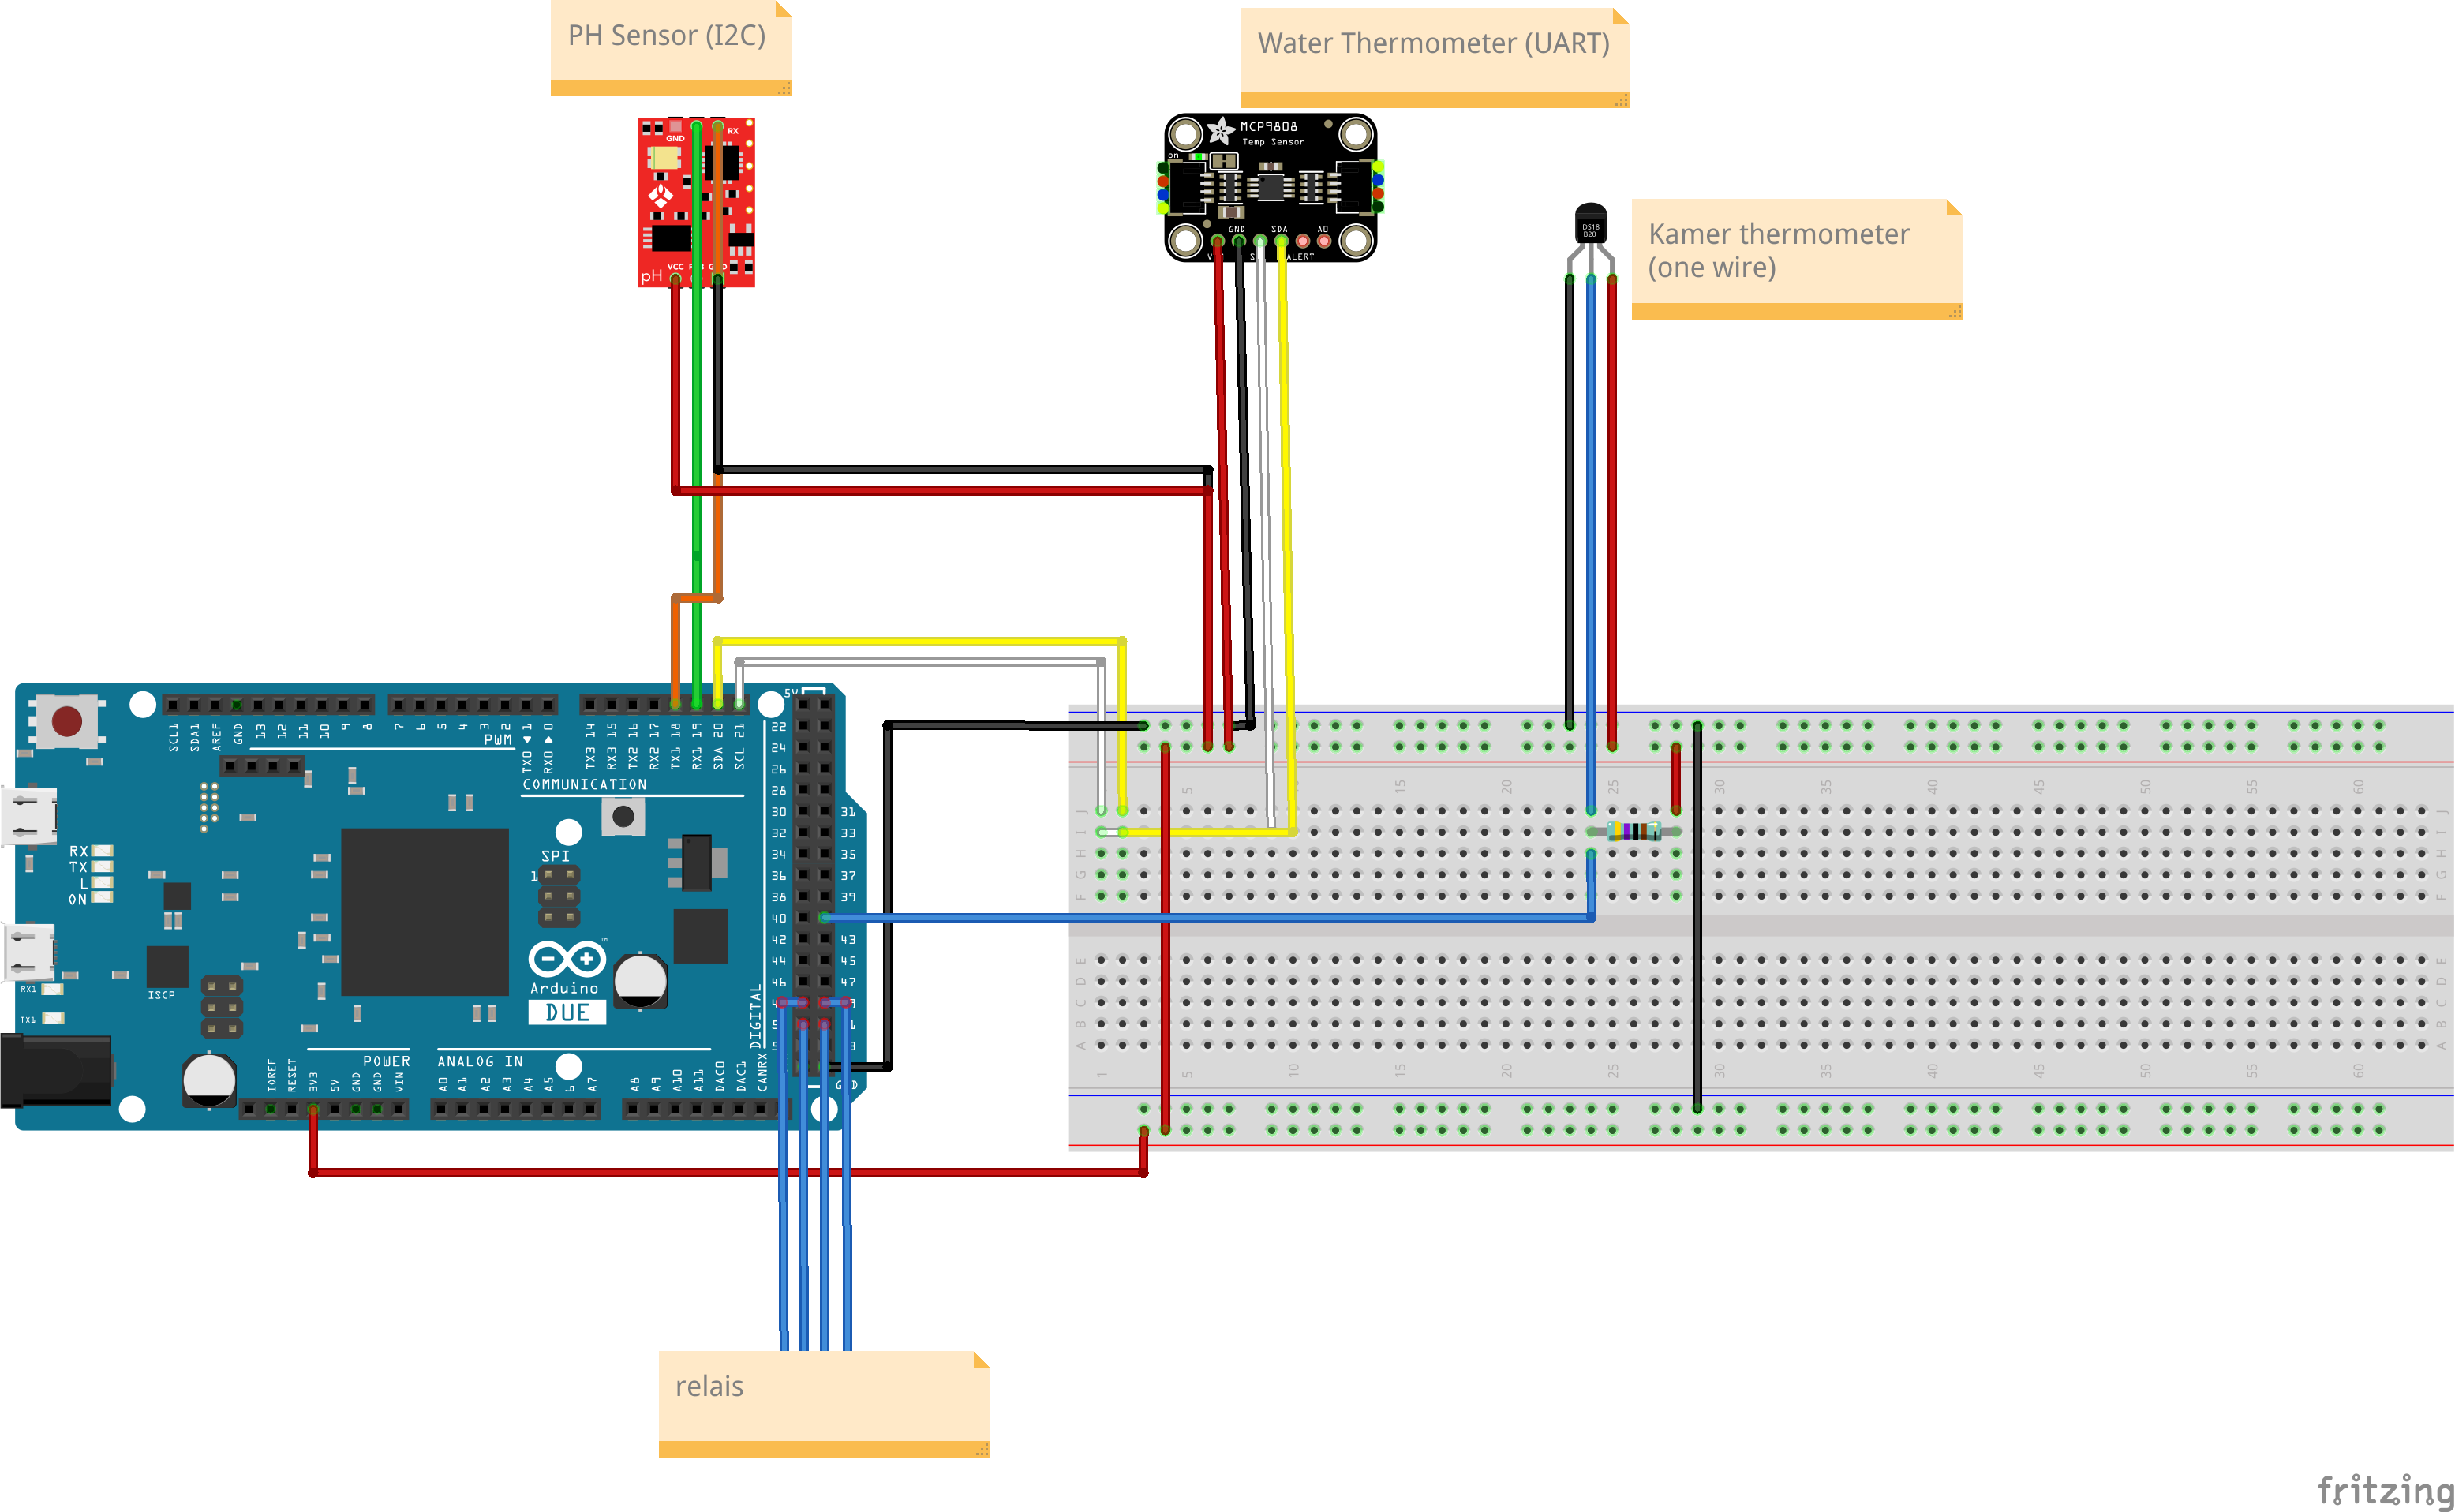
\includegraphics[width=0.9\textwidth]{Images/hardware_sketch_fritzing.png}
  \caption{Fritzing Hardware Diagram}
  \label{fig:hardware_sketch_fritzing}
\end{figure}
% TODO: Korte beschrijving over het diagram.


\section{Software}
Het systeem wordt ontwikkeld met Visual Studio Code. Het \turtleguard systeem zal voornamelijk worden geïmplementeerd in Python. De sensoren en actuatoren worden geïmplementeerd in C++.

De code zal voornamelijk worden geprogrammeerd op een object-georiënteerde en aspect-georiënteerde wijze. 
Daarnaast wordt het controle systeem geïmplementeerd volgens het Functional Reactive Programming principe.
De koppeling tussen Python en C++ zal worden gedaan via pybind, omdat dit een modern en relatief simpele koppeling is tussen C++ en Python.

Het systeem zal de volgende klassenstructuur hebben.
% TODO: Klassendiagram
\begin{figure}[h]
  \centering
  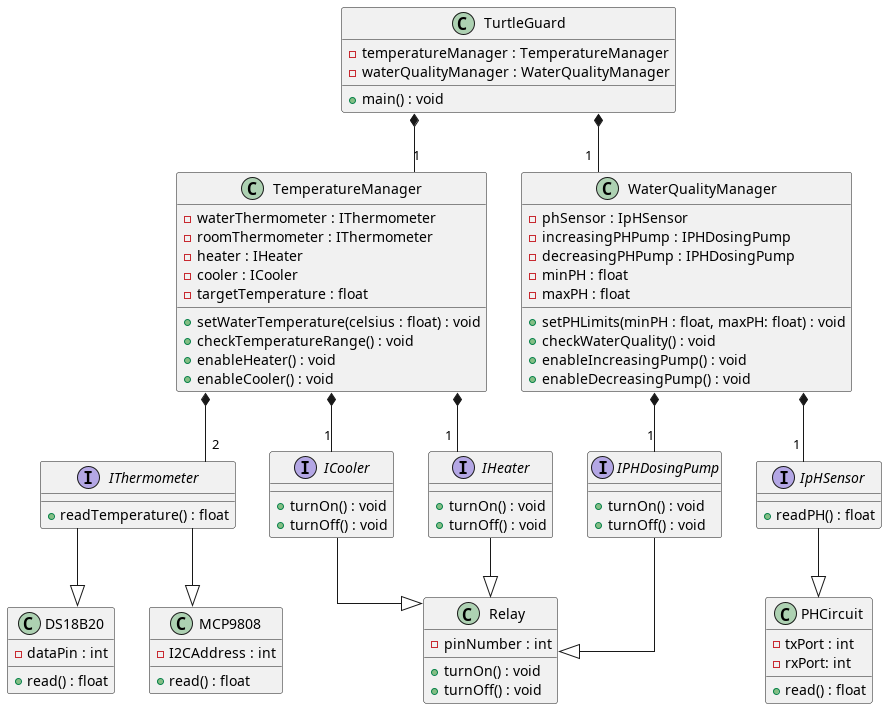
\includegraphics[width=0.8\textwidth]{Images/classdiagram.png}
  \caption{\turtleguard Klassendiagram}
  \label{fig:classdiagram}
\end{figure}

\par \smallskip
Er zijn verschillende flows binnen het systeem. De simpelste is de 'main' flow. Dit is simpelweg de entrypoint van het programma.
Dit entrypoint maakt gebruik van de twee 'managers' binnen het systeem, welke beide op zich aparte delen van het systeem 'managen'.
Dit zijn de Temperatuur-manager en de Waterkwaliteits-manager. 
Voor het gemak is een activity diagram gemaakt voor elk van deze systemen. De managers zullen verder worden toegelicht in hoofdstuk \ref{sec:tempmgr} en \ref{sec:wqmgr}. 

% Todo: activity diagram

\begin{figure}[H]
  \centering
  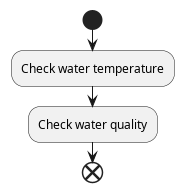
\includegraphics[width=0.3\textwidth]{Images/ActivityDiagram.png}
  \caption{\turtleguard Activity Diagram}
  \label{fig:activitydiagram}
\end{figure}

\subsection{Temperatuur-manager}
\label{sec:tempmgr}
De temperatuur manager is verantwoordelijk voor het meten en waarborgen van de correcte temperaturen binnen het \turtleguard systeem.
Op basis van omgevingstemperatuur en watertemperatuur worden het verwarmingselement en het verkoelingselement aangestuurd.
De gebruiker stelt vooraf een ideale temperatuur in. Het systeem zorgt er voor dat de temperatuur van het aquarium binnen 3\textdegree c van de ideale temperatuur blijft.
Er is gekozen voor een waarde van 3 \textdegree c, omdat dit nog volledig comfortabel is voor de muskus schildpad. Muskus schildpad hebben een voorkeur aan temperaturen van x tot x.
De werking van het systeem staat beschreven in het activity diagram hier onder.

\begin{figure}[H]
  \centering
  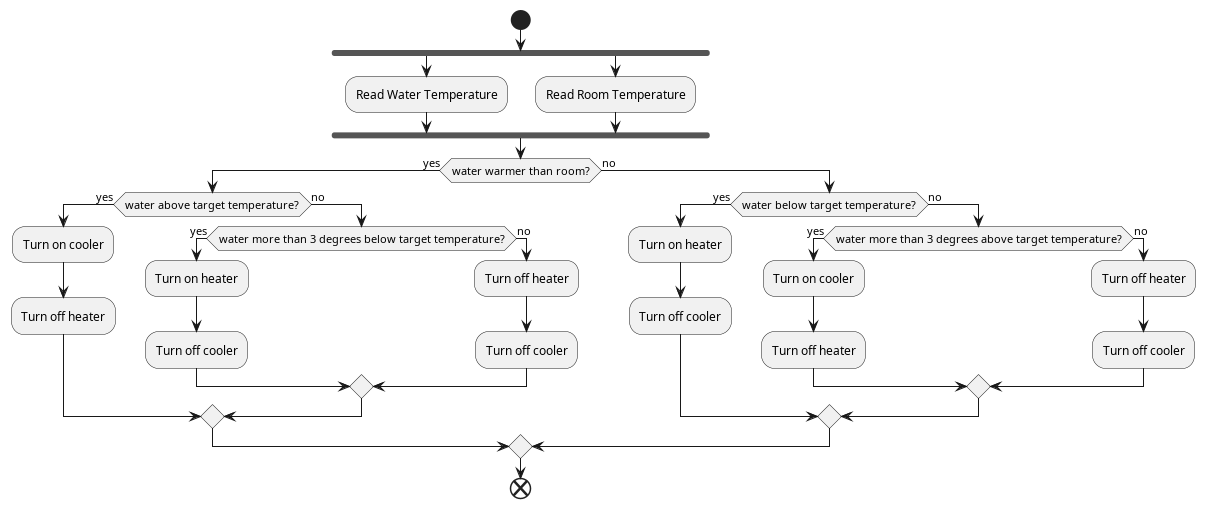
\includegraphics[width=0.9\textwidth]{Images/ActivityDiagramTemp.png}
  \caption{\turtleguard Temperatuur Manager Activity Diagram}
  \label{fig:activitydiagramtemperature}
\end{figure}

\subsection{Waterkwaliteits-manager}
\label{sec:wqmgr}
De waterkwaliteit manager is verantwoordelijk voor het waarborgen van een juiste pH waarde. 
Dat wordt gedaan door middel van twee doseringspompen, in combinatie met een pH sensor.
Deze doseringspompen pompen (schildpad-veilige) chemicaliën in het water, welke de pH kunnen verhogen of verlagen.
De pompen worden aangesloten op het systeem via een relais, welke de pompen aan- of uitzetten.
De werking van dit systeem staat beschreven in het volgende activity diagram. 
\begin{figure}[H]
  \centering
  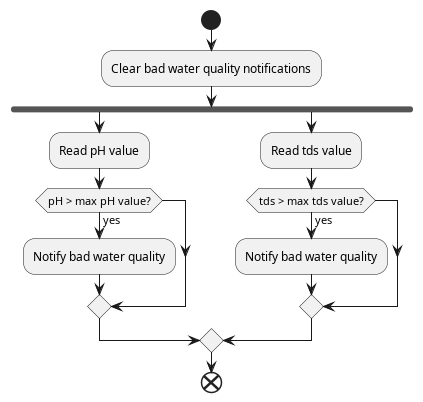
\includegraphics[width=0.5\textwidth]{Images/ActivityDiagramQuality.png}
  \caption{\turtleguard Water Quality Activity Diagram}
  \label{fig:activitydiagram}
\end{figure}

\chapter{Testplan}
\section{Risicoanalyse}
\subsection{Risico's}
Er zijn verschillende risico's die zich kunnen opdoen binnen het systeem indien deze niet (correct) getest wordt.
Als het systeem verkeerde sensor data binnen krijgt, zal het systeem daar onjuist op reageren. Dit kan vervolgens verergeren en uit de hand lopen. 
Denk bijvoorbeeld aan het lezen van positieve temperatuur readings als negatief. Om te compenseren voor de 'negatieve' temperaturen, gaat de verwarming aan.
Als zoiets gebeurt zijn de gevolgen potentieel desastreus. De kans dat dit gebeurt is ook vrij hoog als er niet getest is.
\par \smallskip 
Ten tweede kan zich het probleem voordoen data actuators niet reageren op de waardes. 
Als we bijvoorbeeld de verwarming willen activeren, maar deze activeert niet doordat deze niet goed is verbonden, zal het water niet verwarmd worden.
Hoewel de kans hiervoor groot is, zijn de gevolgen minder groot dan bij de verkeerde sensor data. Het gevolg is dat het water niet verwarmd of verkoeld kan worden. 
Afhankelijk van de kamertemperatuur kan dit ongemakkelijk voor de schildpad worden, maar mits het probleem relatief snel opgelost wordt, is het in de meeste gevallen relatief veilig. 
\par \smallskip 
Ook bestaat er een kans dat het systeem volledig vastloopt. Zonder voldoende te testen is deze kans vrij groot en de gevolgen hierbij zijn vergelijkbaar bij niet-activerende actuators. 
Het kan zorgen voor een ongemakkelijke omgeving voor de schildpad, doordat deze niet in zijn ideale temperatuur leeft, maar de schade zal in de meeste gevallen beperkt blijven.
\par \smallskip
Daarnaast kan het voorkomen dat het systeem te langzaam is om in realtime te reageren. Er wordt gewerkt met gelimiteerde hardware, dus dit risico bestaat. 
Doordat het systeem niet extreem complex of groot is, is het risico beperkt. Als de actuatoren niet op tijd reageren op de sensoren, zal dit geen ernstige gevolgen hebben. 
Hierbij wordt wel uitgegaan van een beperkte vertraging. Als het systeem er vijf minuten over doet om te reageren op een temperatuursverandering, of zelfs een uur, is dit geen grote ramp.
Water reageert immers uit zichzelf wat vertraagd op temperatuursveranderingen. Pas bij extreem grote vertragingen zal dit merkbare gevolgen kunnen hebben, maar zulke vertragingen zijn zeer onwaarschijnlijk.
\par \smallskip 
Binnen het project bestaat er ook een aannemelijke kans voor tijdsnood. Er is een gelimiteerde tijd met daarbij harde deadlines. 
Als deze om wat voor redenen niet gehaald worden, zijn de gevolgen groot voor het project. 

\subsection{Risico Matrix}
\begin{table}[h]
  \centering
  \begin{tabular}{|c|c|c|}
    \hline
    \textbf{Risico} & \textbf{Kans} & \textbf{Impact} \\
    \hline 
    Verkeerde sensor data  & \cellcolor{red} Groot & \cellcolor{red} Groot \\
    \hline 
    Niet activerende actuators & \cellcolor{red} Groot & \cellcolor{orange} Medium \\
    \hline 
    Crashes &\cellcolor{orange} Medium &\cellcolor{red} Medium  \\  
    \hline
    Weinig tijd &\cellcolor{orange} Medium &\cellcolor{red} Groot  \\ 
    \hline
    Vertraagde reacties &\cellcolor{green} Klein &\cellcolor{green} Klein  \\  
    \hline
  \end{tabular}
  \caption{Risicomatrix}
  \label{tab:risicomatrix}
\end{table}

\section{Kwaliteit}
Aan de hand van de kenmerken gedefinieerd in ISO 25010 wordt dit testplan samengesteld, om zo vast te kunnen stellen dat het systeem werkt naar behoren en voldoet aan de kwaliteitseisen.
In onderstaande tabel wordt beschreven hoe elk kenmerk wordt toegepast binnen het testplan om te zorgen dat het systeem hieraan voldoet.

\begin{table}[h]
  \centering
  \begin{tabularx}{\textwidth}{|l|X|}
    \hline
    \textbf{Kenmerk} & \textbf{Omschrijving} \\
    \hline 
    \textbf{Functionaliteit} & Testen van de correcte werking van de sensoren en actuatoren, inclusief pH, TDS en temperatuurmetingen. \\ 
    \hline
    \textbf{Betrouwbaarheid} & Evalueren van de stabiliteit en nauwkeurigheid van het systeem, met focus op foutafhandeling. \\ 
    \hline
    \textbf{Bruikbaarheid} & Valideren van de gebruiksvriendelijkheid van de gebruikersinterface en de leesbaarheid van de sensorgegevens. \\ 
    \hline
    \textbf{Prestaties} & Beoordelen van de reactiesnelheid van het systeem en de verwerkingssnelheid van de sensordata. \\
    \hline
    \textbf{Onderhoudbaarheid} & Beoordelen van de modulariteit en documentatie van de code voor toekomstige aanpassingen. \\
    \hline
    \textbf{Compatibiliteit} & Vaststellen van de compatibiliteit van het systeem met verschillende hardwarecomponenten. \\
    \hline
    \textbf{Beveiliging} & Aandacht voor het voorkomen van ongeautoriseerde toegang tot het systeem, hoewel dit een lagere prioriteit heeft. \\
    \hline
  \end{tabularx}
  \caption{ISO 25010 Kenmerken}
  \label{tab:25010_specs}
\end{table}


Voor het \turtleguard systeem is functionaliteit en betrouwbaarheid het belangrijkste punt. 
Het systeem moet goed werken en mag niet zomaar kapot gaan, omdat de gezondheid van de schildpad hiervan afhankelijk is.
Beveiliging is daarentegen niet belangrijk. Het systeem gaat immers niet met gevoelige data aan de gang. Het regelt simpelweg het water van een schildpad.

\begin{table}[h]
  \centering
  \begin{tabularx}{\textwidth}{|l|X|X|X|X|X|}
    \hline
    \textbf{Kwaliteitskenmerken} & \textbf{Relatief \newline belang \newline (\%)} & \textbf{Hardware \newline unit test} & \textbf{Software \newline unit test} & \textbf{HW/SW \newline integratietest} & \textbf{Systeemtest} \\
    \hline 
    Functionaliteit & 30\% & ++ & ++ &  &  \\ 
    \hline
    Betrouwbaarheid & 30\% & ++ & ++ &  & ++ \\ 
    \hline
    Bruikbaarheid & 15\% &  &  &  & ++ \\ 
    \hline
    Prestaties & 15\% &  &  & ++ &  \\ 
    \hline
    Onderhoudbaarheid & 5\% &  &  &  & + \\ 
    \hline
    Compatibiliteit & 5\% &  &  &  & + \\ 
    \hline
    Beveiliging & 0\% &  &  &  &  \\ 
    \hline
  \end{tabularx}
  \caption{ISO 25010 Prioriteiten}
  \label{tab:25010_priorities}
\end{table}

%De relatieve belangrijkheid in de tabel is gebaseerd op de specifieke behoeften van dit project. "Functionaliteit" en "Betrouwbaarheid" zijn het meest cruciaal, elk met een gewicht van 25\%. Dit komt omdat het systeem niet alleen correct moet functioneren, maar ook betrouwbaar moet zijn om het welzijn van de waterschildpadden te waarborgen. "Bruikbaarheid" en "Prestaties" volgen met elk 15\%, aangezien het systeem gebruiksvriendelijk en responsief moet zijn. "Onderhoudbaarheid" en "Compatibiliteit" zijn ook belangrijk maar in mindere mate, vandaar de 10\%. "Beveiliging" heeft een belangrijkheid van 0\% omdat het systeem niet is verbonden met het internet en het primaire risico fysieke manipulatie is, wat buiten de scope van dit project valt.

% Het belangrijkste punt aan \turtleguard is dat het betrouwbaar is. Zodra het product geïnstalleerd is, wil je dat het gewoon werkt en dat het blijft werken. Het laatste wat je wil is dat het verwarmingselement stopt met werken tijdens lunchtijd.
% Daarnaast is het ook belangrijk dat het systeem makkelijk is te installeren en te gebruiken. Het gehele doel is immers om het leven makkelijker te maken en tijd te besparen, niet het tegenovergestelde.
% Daarom zijn de drie belangrijkste punten, gedefinieerd onder ISO 25010, als volgt:
% \begin{enumerate}
%   \item Betrouwbaarheid
%   \item Bruikbaarheid
%   \item Overdraagbaarheid
% \end{enumerate}

\section{Unit Tests}

\subsection{Water thermometer}

\begin{tcolorbox}[colback=white, colframe=black, title=Beschrijving van de Unit]
Deze unit test richt zich op het meten van de werking en nauwkeurigheid van de water temperatuursensor (DS18B20). 
\end{tcolorbox}

\begin{tcolorbox}[colback=white, colframe=black, title=Test Doel]
Verifiëren dat de water temperatuursensor nauwkeurige en betrouwbare metingen levert.
\end{tcolorbox}

\begin{tcolorbox}[colback=white, colframe=black, title=Test Motivatie]
Het waarborgen van de nauwkeurigheid van de water temperatuursensor is cruciaal voor het welzijn van de schildpadden en de algehele betrouwbaarheid van het \turtleguard-systeem.
Met deze test kan worden getest of de sensor op de juiste manier is geïmplementeerd en hij correcte waardes teruggeeft,
Als er een verkeerde temperatuur wordt uitgelezen, kan het systeem de temperatuur niet goed regelen. De kans bestaat dat het water dan te ver koelt of verwarmt. 
Beide kunnen ziektes en andere gezondheidsproblemen opwekken bij de schildpad.
\end{tcolorbox}

\begin{tcolorbox}[colback=white, colframe=black, title=Test Criteria]
  % wanneer kan de test uitgevoerd worden?
  \begin{itemize}
    \item De sensor is verbonden zoals beschreven in de hardware schetsen 
    \item De code om met de sensor te communiceren is opgezet 
  \end{itemize}
\end{tcolorbox}



\begin{tcolorbox}[colback=white, colframe=black, title=Test Stappen]
  \begin{enumerate}
    \item Dompel de sensor onder in een bak met water 
    \item Meet de temperatuur van de bak met water met een thermometer, waarvan bekend is dat deze accuraat is 
    \item Noteer de water temperatuur uitgelezen via het \turtleguard systeem. 
    \item Vergelijk de twee waardes. 
    \item Herhaal het experiment driemaal met een tussenpozen van 15 minuten. 
  \end{enumerate}
\end{tcolorbox}

\begin{tcolorbox}[colback=white, colframe=black, title=Slagingscriteria]
De test wordt als geslaagd beschouwd als de uitvoer van de sensor binnen 0.5 \textdegree c van de bekende temperatuur ligt.
\end{tcolorbox}


\subsection{pH Sensor}

\begin{tcolorbox}[colback=white, colframe=black, title=Beschrijving van de Unit]
Deze unit test richt zich op het meten van de werking en nauwkeurigheid van de pH sensor(EZO\texttrademark pH Circuit). 
\end{tcolorbox}

\begin{tcolorbox}[colback=white, colframe=black, title=Test Doel]
Het doel van deze test is het verifiëren dat de ph sensor de juiste waardes levert.
\end{tcolorbox}

\begin{tcolorbox}[colback=white, colframe=black, title=Test Motivatie]
Het waarborgen van de nauwkeurigheid van de pH-sensor is cruciaal voor het welzijn van de schildpadden en de algehele betrouwbaarheid van het \turtleguard-systeem.
Met deze test kan worden getest of de sensor op de juiste manier is geïmplementeerd en hij correcte waardes teruggeeft,
Als de sensor een verkeerde waarde afgeeft, kan het zijn dat het systeem het water een te hoge of te lage pH-waarde geeft, wat gezondheidsproblemen kan opleveren bij de schildpad.
\end{tcolorbox}

\begin{tcolorbox}[colback=white, colframe=black, title=Test Criteria]
  % wanneer kan de test uitgevoerd worden?
  \begin{itemize}
    \item De sensor is verbonden zoals beschreven in de hardware schetsen 
    \item De code om met de sensor te communiceren is opgezet 
  \end{itemize}
\end{tcolorbox}

\begin{tcolorbox}[colback=white, colframe=black, title=Test Stappen]
  \begin{enumerate}
    \item Vul een bak met water, met een vooraf bekende pH-waarde.
    \item Dompel de sensor onder de bak met water 
    \item Noteer de pH-waarde, uitgelezen via het \turtleguard systeem. 
    \item Vergelijk de twee waardes. 
  \end{enumerate}
\end{tcolorbox}

\begin{tcolorbox}[colback=white, colframe=black, title=Slagingscriteria]
De test wordt als geslaagd beschouwd als de pH-waarde van de sensor binnen 0.05 pH zit van de vooraf bekende pH-waarde.
\end{tcolorbox}


\section{Integratietests}
\subsection{Integratietest: pH dosering pomp}
\begin{tcolorbox}[colback=white, colframe=black, title=Beschrijving van de interface]
  Deze test richt zich op de interface tussen de pH-sensor en de doseringspompen die pH-verhogende en pH-verlagende chemicaliën toevoegen.
\end{tcolorbox}

\begin{tcolorbox}[colback=white, colframe=black, title=Test Doel]
  Het doel van deze test is om te valideren dat de pH-sensor en de doseringspompen correct samenwerken om binnen de gewenste pH grenzen te blijven.
\end{tcolorbox}

\begin{tcolorbox}[colback=white, colframe=black, title=Test Motivatie]
  Een correcte pH-waarde is cruciaal voor de gezondheid van de muskus schildpadden. Het is daarom cruciaal om te zorgen dat de sensor en de pompen perfect samenwerken.
  Als de pH-waarde te hoog of te laag is, kan dit stress en gezondheidsproblemen veroorzaken voor de schildpad.
\end{tcolorbox}

\begin{tcolorbox}[colback=white, colframe=black, title=Test Criteria]
  % wanneer kan de test uitgevoerd worden?
  \begin{itemize}
    \item De pH-sensor en doseringspompen zijn correct aangesloten.
    \item Het systeem is geïnitialiseerd en klaar voor testen.
    \item Er bevindt zich geen schildpad in het aquarium.
  \end{itemize}
\end{tcolorbox}

\begin{tcolorbox}[colback=white, colframe=black, title=Test Stappen]
  \begin{enumerate}
    \item Initialiseer het systeem met een bekende pH-waarde die te laag is.
    \item Monitor de pH-sensor metingen.
    \item Controleer of de doseringspomp voor het verhogen van de pH wordt geactiveerd.
    \item Meet het nieuwe pH-niveau.
    \item Herhaal stappen 1-4, maar met een te hoge pH-waarde om de doseringspomp voor het verlagen van de pH te activeren.
  \end{enumerate}
\end{tcolorbox}

\begin{tcolorbox}[colback=white, colframe=black, title=Slagingscriteria]
  \begin{itemize}
    \item De doseringspomp voor het verhogen van de pH moet worden geactiveerd als het pH-niveau onder het ingestelde punt ligt.
    \item De doseringspomp voor het verlagen van de pH moet worden geactiveerd als het pH-niveau boven het ingestelde punt ligt.
  \end{itemize}
\end{tcolorbox}


\section{Systeemtests}
\subsection{TurtleGuard}
\begin{tcolorbox}[colback=white, colframe=black, title=Beschrijving van de systeemtest]
  Deze test richt zich op de juiste werking tussen de verschillende interfaces van het gehele \turtleguard systeem.
\end{tcolorbox}

\begin{tcolorbox}[colback=white, colframe=black, title=Test Doel]
  Het doel van deze test is het valideren van de werking van het gehele systeem onder verschillende, reële omstandigheden.
\end{tcolorbox}

\begin{tcolorbox}[colback=white, colframe=black, title=Test Motivatie]
  Het is cruciaal om het gehele systeem te testen voordat het in gebruik wordt genomen. Het comfort, maar ook de veiligheid, van de huisdieren zijn afhankelijk van dit systeem.
  Door middel van deze test kan worden vastgesteld dat alle interfaces op de juiste manier met elkaar samenwerken onder realistische omstandigheden. 
\end{tcolorbox}

\begin{tcolorbox}[colback=white, colframe=black, title=Test Criteria]
  \begin{itemize}
    \item Alle hardware moet vooraf correct aangesloten zijn.
    \item De sensoren dienen geplaatst te zijn. Water sensoren moeten in het water zitten.
    \item De voorgaande tests moeten succesvol afgerond zijn. 
    \item Er dient geen schildpad geplaatst te zijn in het aquarium gedurende de test.
    \item De correcte pH en temperatuur grenswaardes zijn ingesteld.
  \end{itemize}
\end{tcolorbox}

\begin{tcolorbox}[colback=white, colframe=black, title=Test Stappen]
  \begin{enumerate}
    \item Controleer of alle componenten juist zijn verbonden.
    \item Controleer of de pH en temperatuur waardes juist zijn ingesteld. 
    \item Start het systeem.
    \item Observeer het systeem onder verschillende (kamer) temperaturen en met verschillende pH waardes. 
    \item Verifieer of het aquarium binnen de vooraf ingestelde waardes blijft.
  \end{enumerate}
\end{tcolorbox}

\begin{tcolorbox}[colback=white, colframe=black, title=Slagingscriteria]
  De test wordt als geslaagd beschouwd als het systeem gedurende de hele test binnen de veilige en comfortabele grenzen is gebleven.
\end{tcolorbox}


\chapter{Deliverables}

\chapter{Planning}


\chapter{Begrippen}
\begin{acronym}
\acro{TDS}{Total Dissolved Solids}
\acro{ppm}{Parts Per Million}
\end{acronym}


\chapter{Bibliografie}
\nocite{*} % This includes all entries from the .bib file, even if they're not cited in the document
\begingroup
\renewcommand{\chapter}[2]{} % Removes the 'Chapter' heading
\renewcommand{\addcontentsline}[3]{} % Prevents adding this specific entry to TOC
\bibliographystyle{apacite}
\bibliography{bronnen}
\endgroup

\chapter{Bijlagen}

\end{document}